% !TEX root = developer.tex

\chapter{Introduction}\label{chapter:intro}

\section{Overview}
\label{sec:intro:overview}

The \sstmacro software package provides a simulator for large-scale parallel computer architectures.
\sstmacro is a component within the Structural Simulation Toolkit (SST).
SST itself provides the abstract discrete event interface.
\sstmacro implements specifically a coarse-grained simulator for distributed-memory applications. 

The simulator is driven from either a trace file or skeleton application. 
Simulation can be broadly categorized as either off-line or on-line.
Off-line simulators typically first run a full parallel application on a real machine,
recording certain communication and computation events to a simulation trace.
This event trace can then be replayed post-mortem in the simulator.

For large, system-level experiments with thousands of network endpoints, high-accuracy cycle-accurate simulation is not possible,
or at least not convenient.
Simulation requires coarse-grained approximations to be practical.
\sstmacro is therefore designed for specific cost/accuracy tradeoffs.

The developer's manual broadly covers the two main aspects of creating new components.
\begin{itemize}
\item Setting up components to match the \inlinecode{Connectable} interface linking components together via ports and event handlers
\item Registering components with the factory system to make them usable in simulation input files
\end{itemize}

\section{What To Expect In The Developer's Manual}
The developer's manual is mainly designed for those who wish to extend the simulator or understand its internals.
The user's manual, in contrast, is mainly designed for those who wish to perform experiments with \emph{new} applications using \emph{existing} hardware models.
The user's manual therefore covers building and running the core set of SST/macro features.
The developer's manual covers what you need to know to add new features.
The SST design is such that external components are built into shared object \inlinecode{.so} files,
loading them into the simulator core without having to recompile the core itself.

\section{Thousand Foot View of Discrete Event Simulation}
Ignoring the complexities of parallel discrete event simulation (PDES), 
discrete even simulation works with a very simple set of abstractions.
Implementing a discrete event simulation requires components, links, and events (Figure~\ref{fig:desCore}).
Components (or agents) perform operations. Components create, send, and receive events - and that's basically all they do. 
In one example, each component could represent a compute node in the system.
Links between components could represent actual, physical links in the network.
The events sent on links are MPI messages.

Time only advances in the simulator \emph{between} events.
It is important to distinguish virtual time (the time being estimated by simulation) from wall clock time (the real time the simulator is running).
Links have an associated latency (delay) and are scheduled by the simulation core to arrive at components at a specific time.
This list of event arrivals at components creates an event queue (more precisely event heap) that is sorted by soonest event time.
As events are popped off the heap, the simulation clock is updated.
The component handles the incoming event, which could cause the component to create and send new events to other components.
The simulation ends when all components quiesce, with no more events active in the system.

Components never interact directly (i.e. a component can never have a shared-memory pointer to another component).
Components can only interact with links.
All information transmitted between components must be encapsulated as an abstract event.
In parallel discrete event simulation, the challenge is both delivering events through distributed memory and maintaining a consistent virtual clock.
Without proper synchronization, one component could have its virtual clock advance too quickly.
It then might receive events from other components with timestamps in the past,
creating an event order violation.
As long as developers obey the component, link, and event abstractions, all of these complexities are handled automatically by the simulation core.

\begin{figure}
\centering
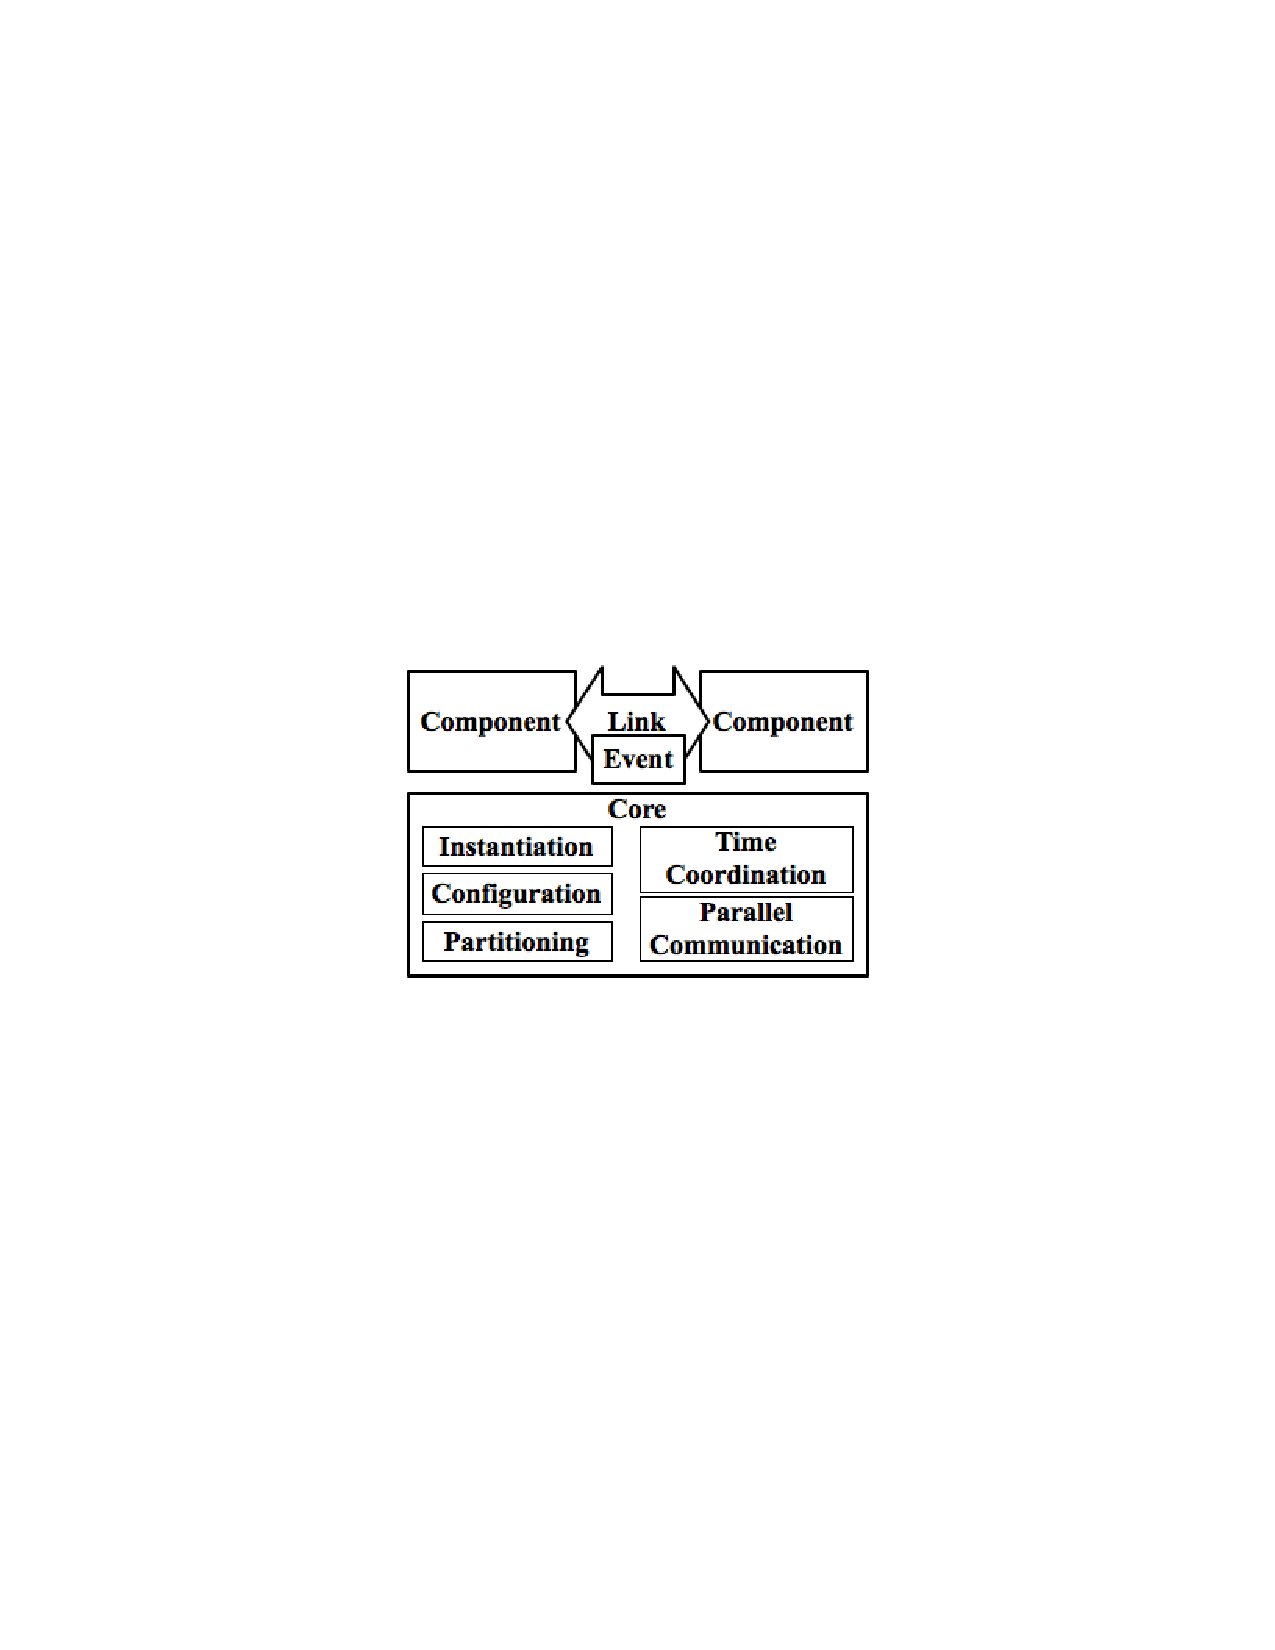
\includegraphics[width=0.3\textwidth]{figures/desCore}

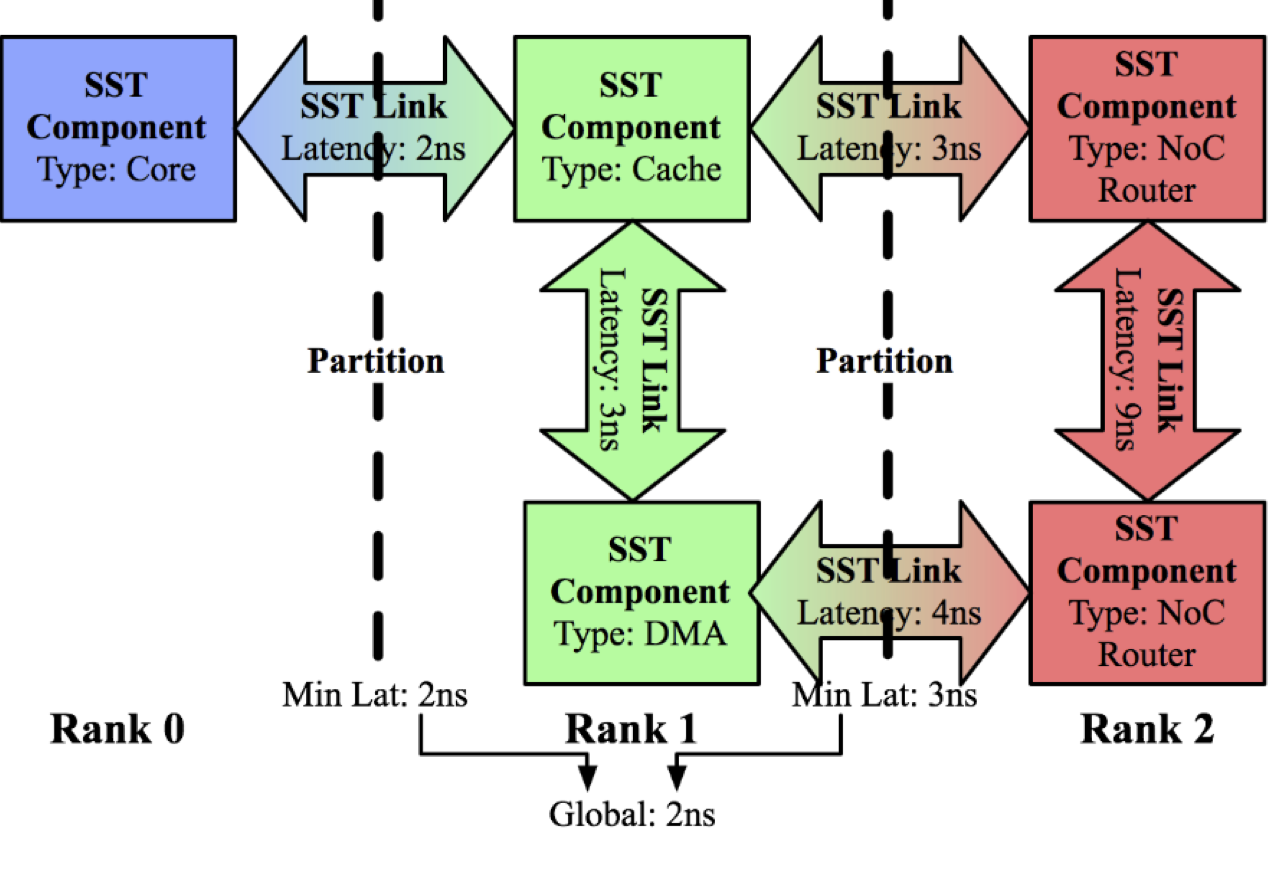
\includegraphics[width=0.5\textwidth]{figures/pdesCore}
\caption{Basic structure of discrete event simulation linking components with links (of a given latency). Link delays advance the simulation clock, which is coordinated by the discrete event core. Parallel discrete event simulation involves placing components on different MPI ranks. The link objects (and simulator core) are responsible for delivering events across MPI boundaries.}
\label{fig:desCore}
\end{figure}

\section{Use of C++}
SST/macro (Structural Simulation Toolkit for Macroscale) is a discrete event simulator designed for macroscale (system-level) experiments in HPC. 
SST/macro is an object-oriented C++ code that makes heavy use of dynamic types and polymorphism.
While a great deal of template machinery exists under the hood, nearly all users and even most developers will never actually need to interact with any C++ templates.
Most template wizardry is hidden in easy-to-use macros.
While C++ allows a great deal of flexibility in syntax and code structure, we are striving towards a unified coding style.

Boost is no longer required or even used.
Some C++11 features like \inlinecode{unordered_map} and \inlinecode{shared_ptr} are used heavily throughout the code.

\begin{figure}
\centering
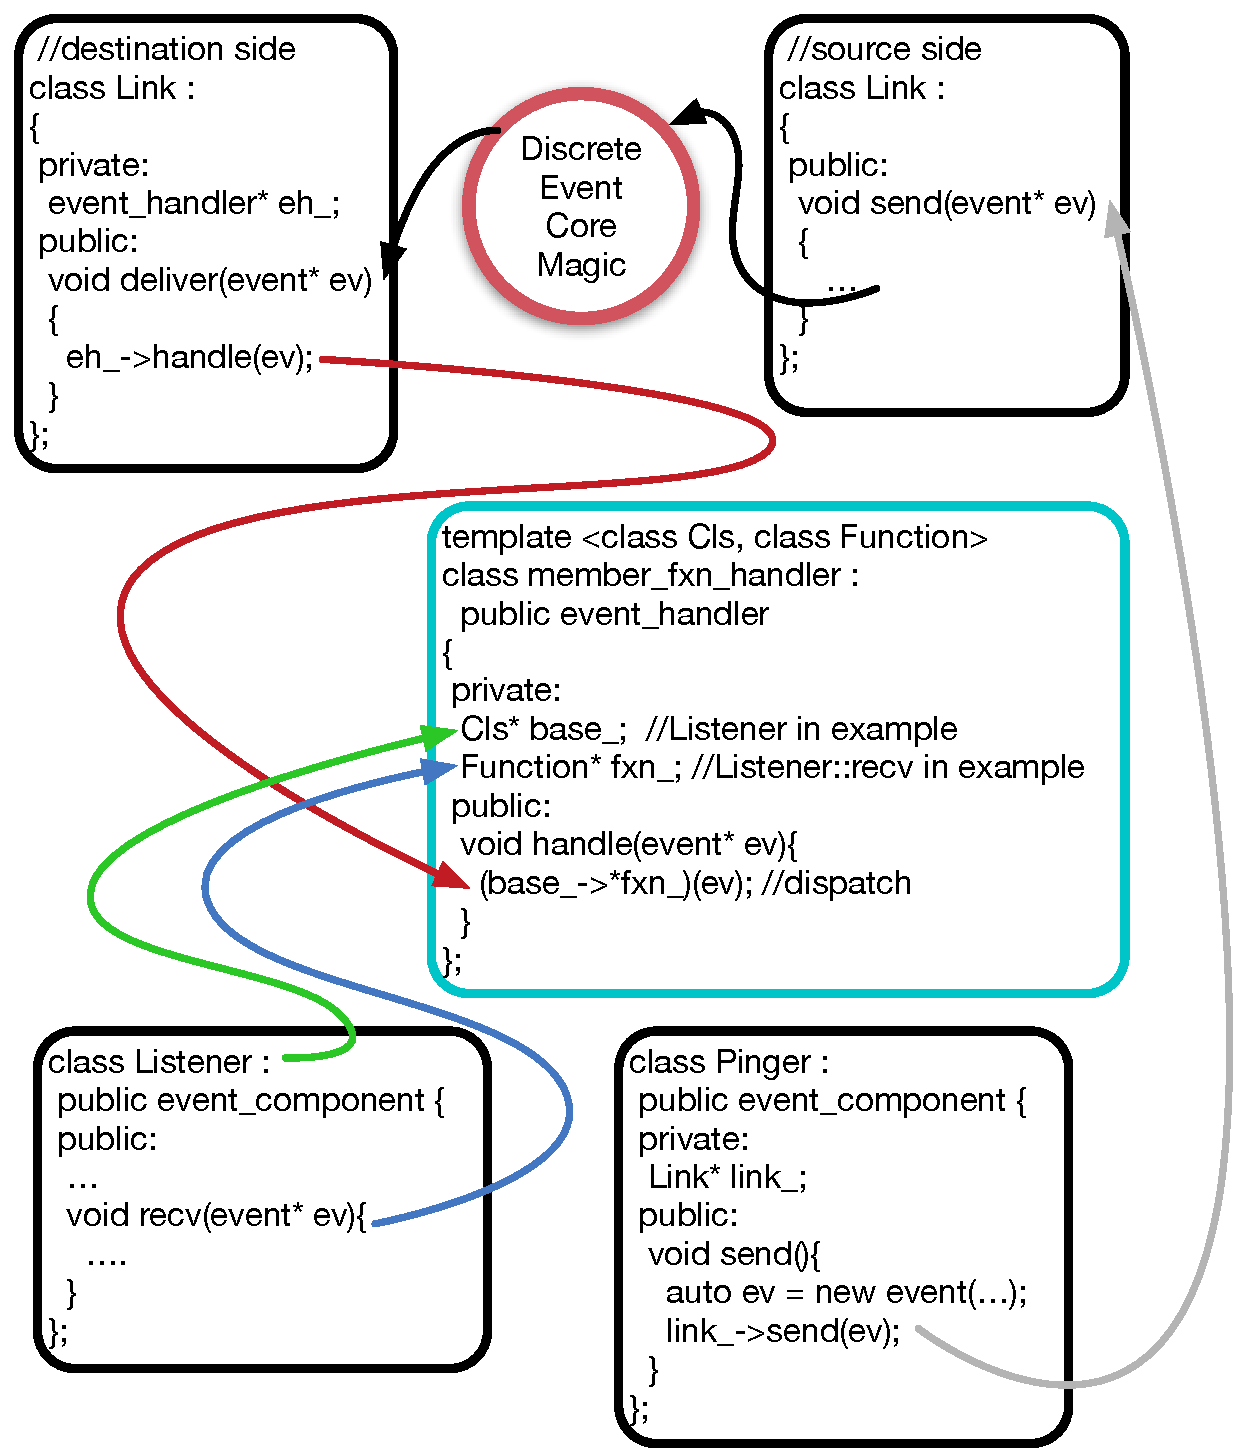
\includegraphics[width=0.8\textwidth]{figures/EventHandler}
\caption{Structure of the simulation connecting components with links and event handlers.}
\label{fig:abstractHandlers}
\end{figure}

\section{Polymorphism and Modularity}\label{sec:polymorphism}
The simulation progresses with different modules (classes) exchanging events.
In general, when module 1 sends a message to module 2, module 1 only sees an abstract interface for module 2.
The polymorphic type of module 2 can vary freely to employ different physics or congestions models without affecting the implementation of module 1. 
Polymorphism, while greatly simplifying modularity and interchangeability, does have some consequences.
The ``workhorse'' of SST/macro is the base \inlinecode{event}, \inlinecode{Component}, and \inlinecode{EventHandler} classes.
To increase polymorphism and flexibility, every SST/macro module that receives events does so via the generic function

\begin{CppCode}
void handle(event* ev){
...
}
\end{CppCode}
The prototype therefore accepts \emph{any} event type. 
The interaction of these types is illustrated in Figure~\ref{fig:abstractHandlers}).
Event handlers are created as dispatch wrappers to member functions of an en \inlinecode{Component}.
There are special helper functions and template classes in SST/macro designed to simplify this process.
A \inlinecode{link} is created connecting two components.
An \inlinecode{EventHandler} is created that dispatches to the \inlinecode{Listener::recv} member function.
When events are pushed onto the link by \inlinecode{Pinger},
the simulation core computes the correct link delay.
After advancing virtual simulation time,
the simulation core invokes the event handler, which delivers the event to the \inlinecode{Listener}.

Misusing types in SST/macro is \emph{not} a compile-time error.
The onus of correct event types falls on runtime assertions.
All event types may not be valid for a given module.
A module for the memory subsystem should throw an error if the developer accidentally passes it an event intended for the OS or the NIC.
Efforts are being made to convert runtime errors into compile-time errors.
In many cases, though, this cannot be avoided.
The other consequence is that a lot of dynamic casts appear in the code.
An abstract \inlinecode{event} type is received, but must be converted to the specific message type desired.
NOTE: While \emph{some} dynamic casts are sometimes very expensive in C++ (and are implementation-dependent),
most SST/macro dynamic casts are simple equality tests involving virtual table pointers and relatively low overhead.

While, SST/macro strives to be as modular as possible, allowing arbitrary memory, NIC, interconnect components,
in many cases certain physical models are simply not compatible.
For example, using a fluid flow model for memory reads cannot be easily combined with a packet-based model for the network.
Again, pairing incompatible modules is not a compile-time error.
Only when the types are fully defined at runtime can an incompatibility error be detected.
Again, efforts are being made to convert as many type-usage problems into compiler errors.
We prefer simulation flexibility to compiler strictness, though. 

\section{Most Important Style and Coding Rules}\label{sec:stylerules}
Here is a selection of C++ rules we have tended to follow.  
Detailed more below, example scripts are included to reformat the code style however you may prefer for local editing.
However, if committing changes to the repository, only use the default formatting in the example scripts.
\begin{itemize}
\item snake\_case is used for variable and class names.
\item We use ``one true brace`` style (OTBS) for source files. 
\item In header files, all functions are inline style with attached brackets.
\item To keep code compact horizontally, indent is set to two spaces. Namespaces are not indented.
\item Generally, all if-else and for-loops have brackets even if a single line.
\item Accessor functions are not prefixed, i.e. a function would be called \inlinecode{name()} not \inlinecode{get_name()}, except
where conflicts require a prefix. Functions for modifying variables are prefixed with \inlinecode{set_},
\item We use .h and .cc instead of .hpp and .cpp
\item As much implementation as possible should go in .cc files.
	Header files can end up in long dependency lists in the make system.  
	Small changes to header files can result in long recompiles.
	If the function is more than a basic set/get, put it into a .cc file.
\item Header files with many classes are discouraged.  When reasonable, one class per header file/source file is preferred.
	 Many short files are better than a few really long ones.
\item Document, document, document.  If it isn't obvious what a function does, add doxygen-compatible documentation.
	Examples are better than abstract wording.
\item Use STL and Boost containers for data structures.  Do not worry about performance until much later.
	Premature optimization is the root of all evil. If determined that an optimized data structure is needed,
	please do that after the entire class is complete and debugged.
\item Forward declarations.  There are a lot of interrelated classes, often creating circular dependencies. In addition, you can add up with an explosion of include files, often involving classes that are never used in a given \inlineshell{.cc} file.  For cleanliness of compilation, you will find many \inlineshell{*_fwd.h} files throughout the code. If you need a forward declaration, we encourage including this header file rather than ad hoc forward declarations throughout the code.
\end{itemize}

Since we respect the sensitivity of code-style wars, we include scripts that demonstrate basic usage of the C++ code formatting tool \emph{astyle}.
This can be downloaded from {http://astyle.sourceforge.net}. 
A python script called \inlineshell{fix_style} is included in the top-level bin directory.
It recursively reformats all files in a given directory and its subdirectories.

%\section{Memory Allocation}\label{sec:memalloc}
%To improve performance, custom memory allocation strategies can be employed in C++.
%At present, a global custom \inlinecode{operator new} can be optionally activated which is optimized for large pages and memory pools.
%At present, no class-specific implementation of \inlinecode{operator new} is used.
%However, we may soon implement custom allocation techniques to improve things like cache/TLB efficiency.
%This is the only major change expected to SST/macro that would affect externally developed modules - and even here the expected modifications would be quite small.
%Because custom allocation schemes may be used, all externally developed code should use \inlinecode{operator new}, rather than \emph{not}  \inlinecode{malloc} or \inlinecode{mmap}, unless allocating very large arrays.

